\documentclass[aspectratio=169,11pt]{beamer}

\usetheme{metropolis}
\usepackage{booktabs}
\usepackage{amsmath,amssymb}
\usepackage{graphicx}
\usepackage{subcaption}
\usepackage{xcolor}
\usepackage{pgfplots}
\pgfplotsset{compat=1.18}
\usepackage{tikz}

\graphicspath{{../figures/}}

% Metropolis tweaks
\setbeamercolor{frametitle}{bg=black!85}
\metroset{block=fill}

\title{Attention Plasticity and the Geometry\\of Long-Context Failure}
\author{Viktor Shcherbakov}
\institute{University of Geneva}
\date{2026}

\begin{document}

% ============================================================
\begin{frame}[plain]
\titlepage
\begin{tikzpicture}[remember picture,overlay]
\node[anchor=south east,xshift=-10pt,yshift=10pt] at (current page.south east)
    {\includegraphics[height=1.2cm]{UNIGElogo.pdf}};
\end{tikzpicture}
\end{frame}

% ============================================================
\begin{frame}{The Problem: Claimed vs.\ Effective Context}

\begin{columns}[T]
\begin{column}{0.42\textwidth}
Models advertise 128K+ token windows, yet
\textbf{effective} context falls far short.

\medskip
Benchmarks detect the gap but cannot explain \emph{why}.

\medskip
\textbf{This thesis:} trace the gap to the geometry of attention heads.
\end{column}
\begin{column}{0.56\textwidth}
\begin{tikzpicture}
\begin{axis}[
    width=\textwidth,
    height=0.72\textheight,
    xlabel={Context length (tokens)},
    ylabel={RULER score (\%)},
    xmode=log,
    log basis x=2,
    xtick={4096,8192,16384,32768,65536,131072},
    xticklabels={4K,8K,16K,32K,64K,128K},
    xticklabel style={font=\scriptsize},
    yticklabel style={font=\scriptsize},
    xlabel style={font=\small},
    ylabel style={font=\small},
    ymin=0, ymax=100,
    legend style={font=\tiny, at={(0.02,0.02)}, anchor=south west,
                  draw=none, fill=white, fill opacity=0.8, text opacity=1,
                  row sep=1pt},
    grid=major,
    grid style={gray!30},
    every axis plot/.append style={thick, mark size=1.5pt},
]
% GPT-4 (128K claimed)
\addplot[color={rgb,255:red,0;green,119;blue,187}, mark=*] coordinates {(4096,96.6) (8192,96.3) (16384,95.2) (32768,93.2) (65536,87.0) (131072,81.2)};
% Llama-3.1 70B (128K claimed)
\addplot[color={rgb,255:red,51;green,160;blue,44}, mark=square*] coordinates {(4096,96.5) (8192,95.8) (16384,95.4) (32768,94.8) (65536,88.4) (131072,66.6)};
% Llama-3.1 8B (128K claimed)
\addplot[color={rgb,255:red,204;green,102;blue,0}, mark=triangle*] coordinates {(4096,95.5) (8192,93.8) (16384,91.6) (32768,87.2) (65536,84.7) (131072,77.0)};
% Qwen-2 72B (128K claimed)
\addplot[color={rgb,255:red,148;green,103;blue,189}, mark=diamond*] coordinates {(4096,96.9) (8192,96.1) (16384,94.9) (32768,94.1) (65536,79.8) (131072,53.7)};
% Mistral-v0.2 7B (32K claimed)
\addplot[color={rgb,255:red,214;green,39;blue,40}, mark=pentagon*] coordinates {(4096,93.6) (8192,91.2) (16384,87.2) (32768,75.4) (65536,49.0) (131072,13.8)};
\legend{GPT-4 (128K), Llama-3.1-70B (128K), Llama-3.1-8B (128K),
        Qwen-2-72B (128K), Mistral-v0.2-7B (32K)}
\end{axis}
\end{tikzpicture}
\end{column}
\end{columns}

\end{frame}

% ============================================================
\begin{frame}{Hypothesis: Attention as Content-Based Reranking}

Attention computes a \textbf{ranking} over keys via dot-product scores:
\[
\text{score}(q, k_i) = q^\top k_i = \underbrace{q_{\text{content}}^\top k_{\text{content}}}_{\text{content relevance}} + \underbrace{q_{\text{pos}}^\top k_{\text{pos}}}_{\text{positional bias}}
\]

\bigskip
When position dominates $\Rightarrow$ ranking becomes \textbf{rigid}:
the model ranks by position rather than by content relevance.

\bigskip
\textbf{Hypothesis:} This rigidity is the mechanistic pathway from architecture to effective context failure.

\end{frame}

% ============================================================
\begin{frame}{Research Questions}

\begin{description}
    \item[RQ1] How does position information manifest in the geometry of
    attention heads?
    \begin{itemize}
        \item[\(\to\)] PCA decomposition + Planar rotation model
    \end{itemize}

    \bigskip
    \item[RQ2] Does positional bias functionally constrain attention?
    \begin{itemize}
        \item[\(\to\)] Attention plasticity metric + decay theorem
    \end{itemize}

    \bigskip
    \item[RQ3] Do plasticity profiles correspond to behavioral performance?
    \begin{itemize}
        \item[\(\to\)] Cross-model benchmark correlation + training dynamics
    \end{itemize}
\end{description}

\end{frame}

% ============================================================
\begin{frame}{PCA: Position Dominates Q/K Variance}

\begin{center}
\includegraphics[height=0.50\textheight]{qk-pca/01_pc_roles/figure.png}
\end{center}

\vspace{-0.5em}
\begin{itemize}
    \item PC0 captures $\sim$34\% of Q+K variance (4$\times$ PC1).
    23--32\% of query and 9--20\% of key variance is \textbf{linear in position}.
    \item On PC0: $|r_q| \approx 0.80 > |r_k| \approx 0.49$
    --- but \alert{this is a confound} (PC0 mixes position with Q/K identity).
\end{itemize}

\end{frame}

% ============================================================
\begin{frame}{PCA: What the First Two Components Look Like}

\begin{center}
\includegraphics[height=0.85\textheight]{qk-pca/06_collage_example/figure.png}
\end{center}

\end{frame}

% ============================================================
\begin{frame}{Rotation: Isolating the Bias Mechanism}

\begin{center}
\includegraphics[height=0.50\textheight]{qk-rotation/02_rq_rk_drift_bars/figure.png}
\end{center}

\vspace{-0.5em}
\begin{itemize}
    \item On drift axis $a$: \textbf{asymmetry reverses} ---
    $|r_k^{(a)}| \approx 0.87 > |r_q^{(a)}| \approx 0.74$.
    Keys encode position more strongly than queries.
    \item Parametric bias: $\text{bias\_str} = \mu_Q^a \times \alpha_K$.
    99\% of 3{,}239 heads show recency bias; tight within families.
\end{itemize}

\end{frame}

% ============================================================
\begin{frame}{Attention Plasticity: The Functional Test}

\textbf{Key idea:} Attention is a reranking mechanism. Pairwise comparison is
the atomic unit of ranking.

\bigskip
Given a random query $q$ and two keys $k_i, k_j$, does the query
\emph{content} determine which key ranks higher?

\begin{align*}
p &= \Phi\!\left(\frac{\mu}{\sqrt{v}}\right),
& \text{PP} &= 4\,p\,(1-p)
\end{align*}

\begin{itemize}
    \item $\text{PP} \to 1$: content determines the ranking (plastic)
    \item $\text{PP} \to 0$: position locks the ordering (rigid)
\end{itemize}

\medskip
\textbf{Theorem:} Under linear positional drift, $\text{AP}_t$ decays with
query position $t$. The \emph{rate} of decay is diagnostic.

\end{frame}

% ============================================================
\begin{frame}{Experimental Setup}

\begin{columns}[T]
\begin{column}{0.48\textwidth}
\textbf{Cross-model study (13 models)}
\smallskip
\begin{tabular}{@{}lrl@{}}
\toprule
Family & \# & Context \\
\midrule
Ministral-3 & 3B/8B/14B & 256K \\
Qwen-3 & 0.6B--14B & 128K \\
Llama-3.2 & 1B/3B/11B & 128K \\
\addlinespace
Llama-3.1 & 8B & 128K \\
Mistral-v0.2 & 7B & 32K \\
\bottomrule
\end{tabular}
\end{column}
\begin{column}{0.48\textwidth}
\textbf{Training dynamics}
\begin{itemize}
    \item SmolLM3-3B
    \item 10 checkpoints
    \item Pre-train $\to$ anneal $\to$ LC ext.
    \item 4K $\to$ 32K $\to$ 64K context
\end{itemize}

\bigskip
\textbf{Benchmarks}
\begin{itemize}
    \item LongBench-Pro (7 models)
    \item RULER (2 predecessor models)
\end{itemize}
\end{column}
\end{columns}

\end{frame}

% ============================================================
\begin{frame}{Result: Plasticity Profiles Separate Families}

\begin{columns}[T]
\begin{column}{0.48\textwidth}
\footnotesize
\begin{tabular}{@{}lccc@{}}
\toprule
Family & 0--20\% & 80--100\% & AP$_{\text{drop}}$ \\
\midrule
Ministral-3 & .655--.664 & .571--.592 & \textbf{.07--.08} \\
Qwen-3 & .680--.702 & .512--.540 & \textbf{.16--.19} \\
Llama-3.2 & .658--.703 & .456--.489 & \textbf{.17--.23} \\
\bottomrule
\end{tabular}

\bigskip
Every model declines. The \textbf{rate} separates families:
\begin{itemize}
    \item Ministral: gradual, near-linear
    \item Qwen: steeper, accelerates
    \item Llama: steepest overall
\end{itemize}
\end{column}
\begin{column}{0.50\textwidth}
\includegraphics[width=0.49\textwidth]{attention-plasticity/01_bucket_heatmap_ministral3_14b/figure.png}%
\hfill%
\includegraphics[width=0.49\textwidth]{attention-plasticity/02_bucket_heatmap_qwen3_14b/figure.png}

\vspace{0.3em}
\includegraphics[width=0.49\textwidth]{attention-plasticity/03_bucket_heatmap_llama3.2_3b/figure.png}%
\hfill%
\includegraphics[width=0.49\textwidth]{attention-plasticity/04_bucket_heatmap_llama3.2_11b/figure.png}
\end{column}
\end{columns}

\end{frame}

% ============================================================
\begin{frame}{Result: Per-Head Strategies Differ by Family}

\begin{columns}[T]
\begin{column}{0.31\textwidth}
\centering
\includegraphics[width=\textwidth]{attention-plasticity/05_profile_ministral3_3b/figure.png}\\
\smallskip
\small Ministral-3-3B\\
\footnotesize Tight, homogeneous bundle
\end{column}
\begin{column}{0.31\textwidth}
\centering
\includegraphics[width=\textwidth]{attention-plasticity/06_profile_qwen3_4b/figure.png}\\
\smallskip
\small Qwen-3-4B\\
\footnotesize Large spread
\end{column}
\begin{column}{0.31\textwidth}
\centering
\includegraphics[width=\textwidth]{attention-plasticity/07_profile_llama3.2_3b/figure.png}\\
\smallskip
\small Llama-3.2-3B\\
\footnotesize Steepest decline
\end{column}
\end{columns}

\end{frame}

% ============================================================
\begin{frame}{Result: AP\textsubscript{drop} Predicts LongBench-Pro}

\begin{columns}[T]
\begin{column}{0.45\textwidth}
\small
\begin{tabular}{@{}lrr@{}}
\toprule
Family & AP$_{\text{drop}}$ & LBP \\
\midrule
Ministral & $\sim$0.07 & 30--40 \\
Qwen & $\sim$0.17 & 31--37 \\
Llama & 0.23 & 16 \\
\bottomrule
\end{tabular}

\bigskip
\textbf{Diagnostic outlier:} Ministral-3-3B --- lowest AP$_{\text{drop}}$
(0.072), highest aggregate AP (0.622), but LBP only 30.18.

\smallskip
$\Rightarrow$ Context preservation is good; base capability is the bottleneck.
\end{column}
\begin{column}{0.52\textwidth}
\includegraphics[width=\textwidth]{attention-plasticity/10_ap_drop_vs_lbp/figure.pdf}
\end{column}
\end{columns}

\end{frame}

% ============================================================
\begin{frame}{Result: Training Dynamics --- Three Phases}

\begin{center}
\includegraphics[height=0.48\textheight]{qk-rotation/10_smollm_bias_decomposition/figure.png}
\end{center}

\vspace{-0.5em}
\small
\begin{columns}[T]
\begin{column}{0.32\textwidth}
\textbf{Phase 1 --- Pre-training}\\
Bias doubles (0.009 $\to$ 0.019).\\
AP$_{\text{drop}}$ $\approx$ 0.06 (mild).
\end{column}
\begin{column}{0.32\textwidth}
\textbf{Phase 2 --- LC 4K to 32K}\\
Bias collapses 6$\times$ via $\alpha_K$ flattening.
Short-context AP recovers.
\end{column}
\begin{column}{0.32\textwidth}
\textbf{Phase 3 --- LC 32K to 64K}\\
Bias halves again (total 10$\times$).\\
\alert{But AP$_{\text{drop}}$ \textbf{triples} to 0.16.}
\end{column}
\end{columns}

\end{frame}

% ============================================================
\begin{frame}{Result: Plasticity Trajectory}

\begin{center}
\includegraphics[height=0.55\textheight]{attention-plasticity/09_smollm3_trajectory/figure.pdf}
\end{center}

Short-context plasticity (AP$_{\text{first\,20\%}}$) \textbf{recovers}
during LC extension.

Long-context plasticity (AP$_{\text{last\,20\%}}$) \textbf{continues to
decline}.

The gap (AP$_{\text{drop}}$) triples despite 10$\times$ bias reduction.

\end{frame}

% ============================================================
\begin{frame}{Limitations}

\begin{itemize}
    \item \textbf{Observational, not causal.} Associations between geometry
    and performance, not interventions.

    \item \textbf{3 families, 1 training trajectory.} Limited generalization
    to MoE, hybrids, or larger scales.

    \item \textbf{Pairwise ranking, not softmax weights.} Captures ranking
    quality, not weight allocation.

    \item \textbf{Base vs.\ instruct confound.} Mechanistic metrics on base
    models; benchmarks on instruct variants.

    \item \textbf{Linear drift / Gaussian assumptions.} Empirically
    supported but approximate; non-linear RoPE structure not captured.
\end{itemize}

\end{frame}

% ============================================================
\begin{frame}{Contributions}

\begin{enumerate}
    \item \textbf{Geometric framework.} PCA $\to$ Rotation $\to$ Plasticity
    --- each resolving what the previous leaves open.

    \bigskip
    \item \textbf{Plasticity decay theorem.} Formal proof + Gaussian closed
    form decomposing decay into positional and content components.

    \bigskip
    \item \textbf{Cross-model validation.} AP$_{\text{drop}}$ separates
    families in benchmark order across 13 models.

    \bigskip
    \item \textbf{Bias $\neq$ context.} 10$\times$ bias collapse but
    AP$_{\text{drop}}$ triples. Content signal decay is the underexplored
    dimension.
\end{enumerate}

\end{frame}

% ============================================================
\begin{frame}{Future Work}

\begin{description}
    \item[Interventional] Ablate low-plasticity heads, measure retrieval
    accuracy at distance.

    \medskip
    \item[Content decay] Which mechanism? RoPE rotation accumulation,
    attention sinks, or feature drift?

    \medskip
    \item[Broader models] MoE, attention-SSM hybrids, 70B+ scales.

    \medskip
    \item[Per-length validation] Full per-length LBP/RULER correlation
    across all matched models.
\end{description}

\end{frame}

% ============================================================
\begin{frame}[plain]
\begin{center}
\Huge Thank you

\bigskip
\Large Questions?
\end{center}
\end{frame}

\end{document}
